% Standalone TikZ figure: Policy Gradient and Maximum Entropy Framework
% For Chapter 3: Reinforcement Learning for Parameter Optimization
\documentclass[tikz,border=10pt]{standalone}
\usepackage{tikz}
\usepackage{amsmath}
\usepackage{amssymb}
\usetikzlibrary{arrows.meta, positioning, shapes.geometric, fit, backgrounds, calc, patterns, decorations.pathreplacing, matrix}

\begin{document}
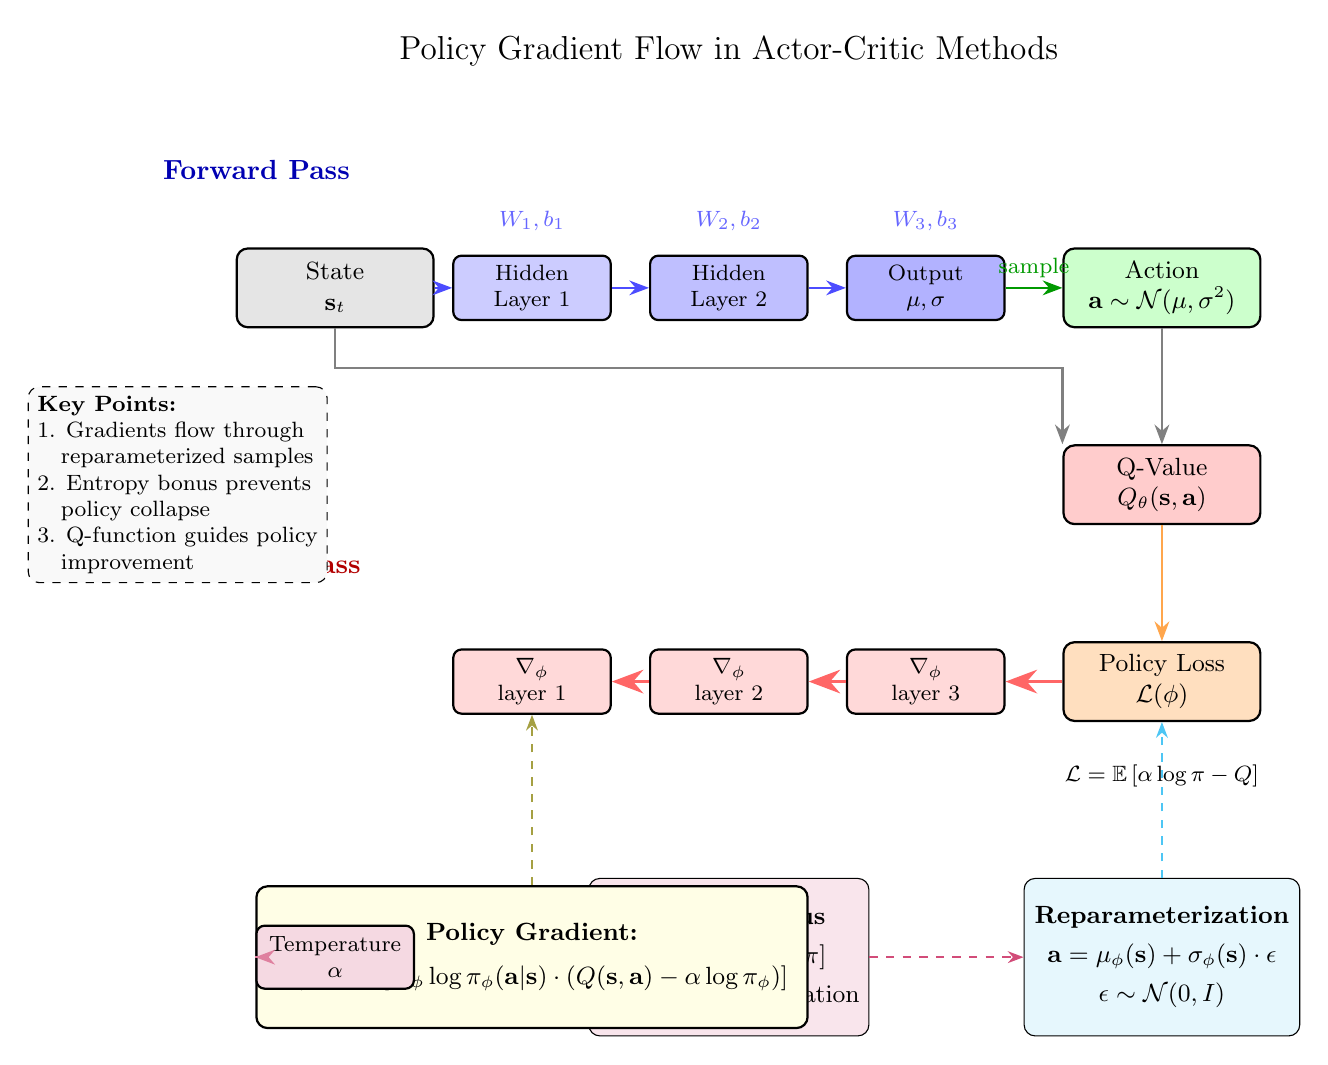
\begin{tikzpicture}[
    every node/.style={font=\small},
    box/.style={rectangle, draw, thick, minimum width=2.5cm, minimum height=1cm, align=center, rounded corners=4pt},
    smallbox/.style={rectangle, draw, thick, minimum width=2cm, minimum height=0.8cm, align=center, rounded corners=3pt, font=\footnotesize},
    arrow/.style={-{Stealth[length=2.5mm]}, thick},
    bigarrow/.style={-{Stealth[length=4mm, width=3mm]}, very thick},
    dashedarrow/.style={-{Stealth[length=2mm]}, thick, dashed},
    label/.style={font=\footnotesize},
    title/.style={font=\bfseries}
]

% ============ MAIN TITLE ============
\node[title, font=\large] at (5, 8) {Policy Gradient Flow in Actor-Critic Methods};

% ============ FORWARD PASS (TOP) ============
\node[title, text=blue!70!black] at (-1, 6.5) {Forward Pass};

% State
\node[box, fill=gray!20] (state) at (0, 5) {State\\$\mathbf{s}_t$};

% Policy network layers
\node[smallbox, fill=blue!20] (layer1) at (2.5, 5) {Hidden\\Layer 1};
\node[smallbox, fill=blue!25] (layer2) at (5, 5) {Hidden\\Layer 2};
\node[smallbox, fill=blue!30] (output) at (7.5, 5) {Output\\$\mu, \sigma$};

% Action sampling
\node[box, fill=green!20] (action) at (10.5, 5) {Action\\$\mathbf{a} \sim \mathcal{N}(\mu, \sigma^2)$};

% Forward arrows
\draw[arrow, blue!70] (state) -- (layer1);
\draw[arrow, blue!70] (layer1) -- (layer2);
\draw[arrow, blue!70] (layer2) -- (output);
\draw[arrow, green!60!black] (output) -- node[above, font=\footnotesize] {sample} (action);

% ============ Q-VALUE COMPUTATION ============
\node[box, fill=red!20] (qvalue) at (10.5, 2.5) {Q-Value\\$Q_\theta(\mathbf{s}, \mathbf{a})$};

\draw[arrow, gray] (state.south) -- ++(0, -0.5) -| (qvalue.north west);
\draw[arrow, gray] (action) -- (qvalue);

% ============ BACKWARD PASS (BOTTOM) ============
\node[title, text=red!70!black] at (-1, 1.5) {Backward Pass};

% Gradient flow boxes
\node[smallbox, fill=red!15] (grad3) at (7.5, 0) {$\nabla_\phi$\\layer 3};
\node[smallbox, fill=red!15] (grad2) at (5, 0) {$\nabla_\phi$\\layer 2};
\node[smallbox, fill=red!15] (grad1) at (2.5, 0) {$\nabla_\phi$\\layer 1};

% Gradient source
\node[box, fill=orange!25] (loss) at (10.5, 0) {Policy Loss\\$\mathcal{L}(\phi)$};

% Loss equation
\node[label, align=center] at (10.5, -1.2) {$\mathcal{L} = \mathbb{E}\left[\alpha \log\pi - Q\right]$};

% Backward arrows (gradient flow)
\draw[bigarrow, red!60] (loss) -- (grad3);
\draw[bigarrow, red!60] (grad3) -- (grad2);
\draw[bigarrow, red!60] (grad2) -- (grad1);

% Connect to Q-value
\draw[arrow, orange!70] (qvalue) -- (loss);

% ============ REPARAMETERIZATION TRICK ============
\node[draw, rounded corners, fill=cyan!10, minimum width=3.5cm, minimum height=2cm, align=center] (reparam) at (10.5, -3.5) {
    \textbf{Reparameterization}\\[3pt]
    $\mathbf{a} = \mu_\phi(\mathbf{s}) + \sigma_\phi(\mathbf{s}) \cdot \epsilon$\\[3pt]
    $\epsilon \sim \mathcal{N}(0, I)$
};

\draw[dashedarrow, cyan!70] (reparam) -- ++(0, 1.5) -- (loss);

% ============ ENTROPY REGULARIZATION ============
\node[draw, rounded corners, fill=purple!10, minimum width=3cm, minimum height=2cm, align=center] (entropy) at (5, -3.5) {
    \textbf{Entropy Bonus}\\[3pt]
    $\mathcal{H}(\pi) = -\mathbb{E}[\log\pi]$\\[3pt]
    Encourages exploration
};

\draw[dashedarrow, purple!70] (entropy.east) -- (reparam.west);

% ============ GRADIENT EQUATION ============
\node[draw, thick, rounded corners, fill=yellow!10, minimum width=7cm, minimum height=1.8cm, align=center] (gradeq) at (2.5, -3.5) {
    \textbf{Policy Gradient:}\\[5pt]
    $\nabla_\phi J = \mathbb{E}\left[\nabla_\phi \log\pi_\phi(\mathbf{a}|\mathbf{s}) \cdot \left(Q(\mathbf{s},\mathbf{a}) - \alpha \log\pi_\phi\right)\right]$
};

% Arrow from gradient equation to backward flow
\draw[dashedarrow, yellow!60!black] (gradeq.north) -- ++(0, 1.5) -| (grad1.south);

% ============ ANNOTATIONS ============
% Annotations for layers
\node[label, text=blue!60, above] at (2.5, 5.6) {$W_1, b_1$};
\node[label, text=blue!60, above] at (5, 5.6) {$W_2, b_2$};
\node[label, text=blue!60, above] at (7.5, 5.6) {$W_3, b_3$};

% Key insight boxes
\node[draw, dashed, rounded corners, fill=gray!5, align=left, font=\footnotesize] at (-2, 2.5) {
    \textbf{Key Points:}\\
    1. Gradients flow through\\
    \quad reparameterized samples\\
    2. Entropy bonus prevents\\
    \quad policy collapse\\
    3. Q-function guides policy\\
    \quad improvement
};

% Temperature parameter
\node[smallbox, fill=purple!15] (alpha) at (0, -3.5) {Temperature\\$\alpha$};
\draw[arrow, purple!50] (alpha) -- (gradeq.west);

\end{tikzpicture}
\end{document}
